\documentclass[tikz,border=8pt]{standalone}
% Shared look for every TikZ diagram. Load with % Shared look for every TikZ diagram. Load with % Shared look for every TikZ diagram. Load with \input{../../tools/tikz-style.tex}
\usepackage[T1]{fontenc}
\usepackage{lmodern}
\renewcommand{\sfdefault}{lmr}  % diagrams use the same serif as the text
\usetikzlibrary{arrows.meta, positioning, shapes.geometric, calc, fit, backgrounds}
\definecolor{cblue}{HTML}{4C78A8}
\definecolor{corange}{HTML}{F58518}
\definecolor{cgreen}{HTML}{54A24B}
\definecolor{cred}{HTML}{E45756}
\definecolor{cpurple}{HTML}{B279A2}
\definecolor{cgrey}{HTML}{6B6B6B}
\tikzset{
  every picture/.style={font=\sffamily, line width=1.2pt},
  box/.style={draw=#1, fill=#1!12, rounded corners=4pt, align=center, inner sep=7pt, minimum height=1.1cm},
  box/.default=cgrey,
  arrow/.style={-{Stealth[length=3mm]}, draw=cgrey, line width=1.4pt},
  title/.style={font=\sffamily\bfseries\Large},
  note/.style={font=\sffamily\small, text=cgrey, align=center},
}
\AtBeginDocument{\hyphenpenalty=10000 \exhyphenpenalty=10000}

\usepackage[T1]{fontenc}
\usepackage{lmodern}
\renewcommand{\sfdefault}{lmr}  % diagrams use the same serif as the text
\usetikzlibrary{arrows.meta, positioning, shapes.geometric, calc, fit, backgrounds}
\definecolor{cblue}{HTML}{4C78A8}
\definecolor{corange}{HTML}{F58518}
\definecolor{cgreen}{HTML}{54A24B}
\definecolor{cred}{HTML}{E45756}
\definecolor{cpurple}{HTML}{B279A2}
\definecolor{cgrey}{HTML}{6B6B6B}
\tikzset{
  every picture/.style={font=\sffamily, line width=1.2pt},
  box/.style={draw=#1, fill=#1!12, rounded corners=4pt, align=center, inner sep=7pt, minimum height=1.1cm},
  box/.default=cgrey,
  arrow/.style={-{Stealth[length=3mm]}, draw=cgrey, line width=1.4pt},
  title/.style={font=\sffamily\bfseries\Large},
  note/.style={font=\sffamily\small, text=cgrey, align=center},
}
\AtBeginDocument{\hyphenpenalty=10000 \exhyphenpenalty=10000}

\usepackage[T1]{fontenc}
\usepackage{lmodern}
\renewcommand{\sfdefault}{lmr}  % diagrams use the same serif as the text
\usetikzlibrary{arrows.meta, positioning, shapes.geometric, calc, fit, backgrounds}
\definecolor{cblue}{HTML}{4C78A8}
\definecolor{corange}{HTML}{F58518}
\definecolor{cgreen}{HTML}{54A24B}
\definecolor{cred}{HTML}{E45756}
\definecolor{cpurple}{HTML}{B279A2}
\definecolor{cgrey}{HTML}{6B6B6B}
\tikzset{
  every picture/.style={font=\sffamily, line width=1.2pt},
  box/.style={draw=#1, fill=#1!12, rounded corners=4pt, align=center, inner sep=7pt, minimum height=1.1cm},
  box/.default=cgrey,
  arrow/.style={-{Stealth[length=3mm]}, draw=cgrey, line width=1.4pt},
  title/.style={font=\sffamily\bfseries\Large},
  note/.style={font=\sffamily\small, text=cgrey, align=center},
}
\AtBeginDocument{\hyphenpenalty=10000 \exhyphenpenalty=10000}

\begin{document}
% Section 9: GPT is the model, ChatGPT is the application built around it (the processor-in-a-laptop analogy).
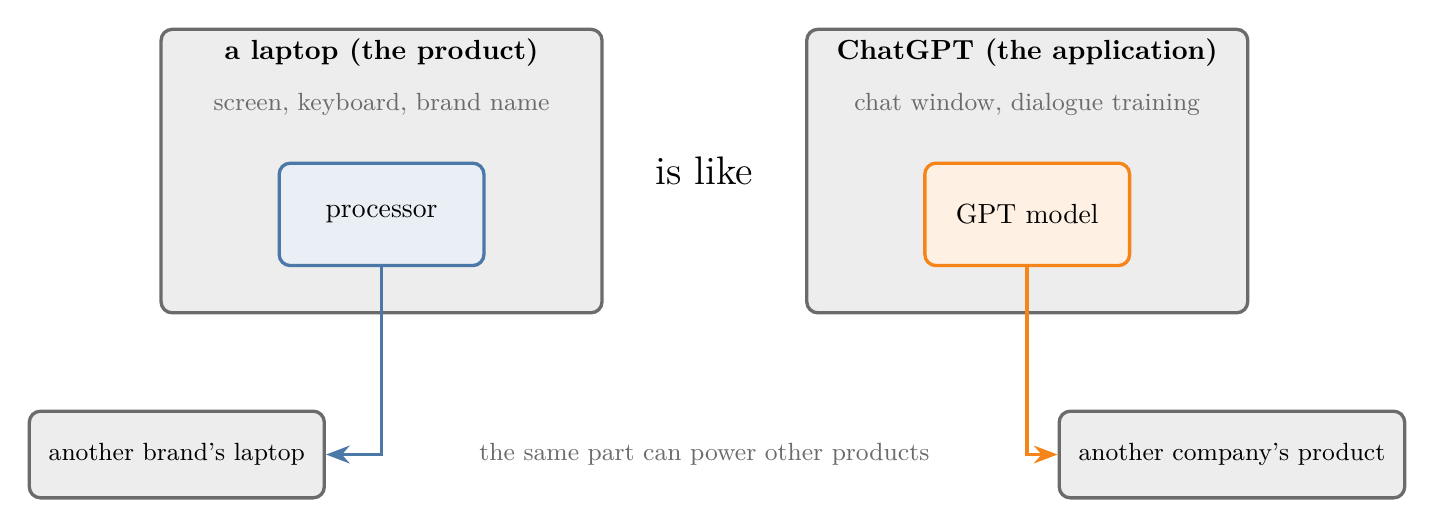
\begin{tikzpicture}
  % left: laptop and its processor
  \node[box=cgrey, minimum width=5.6cm, minimum height=3.6cm] (lap) at (0,0) {};
  \node[font=\sffamily\bfseries, anchor=north] at (lap.north) {a laptop (the product)};
  \node[box=cblue, minimum width=2.6cm, minimum height=1.3cm, font=\sffamily] (cpu) at (0,-0.55) {processor};
  \node[note] at (0,0.85) {screen, keyboard, brand name};
  % right: ChatGPT and the GPT model
  \node[box=cgrey, minimum width=5.6cm, minimum height=3.6cm] (app) at (8.2,0) {};
  \node[font=\sffamily\bfseries, anchor=north] at (app.north) {ChatGPT (the application)};
  \node[box=corange, minimum width=2.6cm, minimum height=1.3cm, font=\sffamily] (gpt) at (8.2,-0.55) {GPT model};
  \node[note] at (8.2,0.85) {chat window, dialogue training};
  \node[font=\sffamily\Large] at (4.1,0) {is like};
  % other products on the same part
  \node[box=cgrey, minimum width=3.2cm, font=\sffamily\small] (o1) at (-2.6,-3.6) {another brand's laptop};
  \draw[arrow, draw=cblue] (cpu.south) |- (o1.east);
  \node[box=cgrey, minimum width=3.2cm, font=\sffamily\small] (o2) at (10.8,-3.6) {another company's product};
  \draw[arrow, draw=corange] (gpt.south) |- (o2.west);
  \node[note] at (4.1,-3.6) {the same part can power other products};
\end{tikzpicture}
\end{document}
